\documentclass[fleqn]{article}
\usepackage[margin=1.5cm]{geometry}   % shrink margins

\newenvironment{answers}{
	\begin{enumerate}
		\setlength{\itemsep}{\bigskipamount}
}{\end{enumerate}}

\newcommand\Item[1][]{ % custom \Item command for block math
  \ifx\relax#1\relax  \item \else \item[#1] \fi
  \abovedisplayskip=0pt\abovedisplayshortskip=0pt~\vspace*{-\baselineskip}
}

\usepackage{amsmath}    % math equation environments
\usepackage{amssymb}    % math symbols such as natural numbers N.

\usepackage[noend]{algpseudocode}		% for algorithms in pseudo code. Usage: \begin{algorithmic}

\usepackage{tikz}	% for diagrams
\usetikzlibrary{positioning}
\usetikzlibrary{arrows.meta}
\usetikzlibrary{calc}

% \usepackage{adjustbox}	% align enumerations containing tall objects to top. Usage: \item\adjustbox{valign=t}{...}

% \usepackage{centernot}	% centers not symbol. Usage: \centernot{...}

% paragraph indentation within enumerations
\usepackage{enumitem}
\setlist{parsep=4pt,listparindent=\parindent}

\title{Intro to Communications \\
\large Homework 2}
\author{Abraham Murciano}

\begin{document}

\maketitle

\section{Error Detecting and Correcting Codes}
\begin{enumerate}[label = Part \arabic*.]
	\item % Part 1
	Given a string of bits 110010101011 and a divisor 11001, when applying the CRC error detection algorithm, the resulting string is 1100101010110000.
	\begin{align*}
							&110010101011\ 0000 \\
		\oplus &\underline{	 110010000000\ 0000 } \\
							&000000101011\ 0000 \\
		\oplus &\underline{	 000000110010\ 0000 } \\
							&000000011001\ 0000 \\
		\oplus &\underline{	 000000011001\ 0000 } \\
							&000000000000\ 0000
	\end{align*}

	\item % Part 2
	The following string of bits was received via Hamming code 111110111011100. There are 15 bits in this string, so there are 4 parity bits and 11 data bits. Here is the string with the parity bits underlined.
	\[1111101\underline{1}101\underline{1}1\underline{00}\]

	The rightmost parity bit is a 0, and it corresponds to the parity of the underlined bits in the following string. Since there are seven 1's in those positions, there must be an error in one of those.
	\[\underline{1}1\underline{1}1\underline{1}0\underline{1}1\underline{1}0\underline{1}1\underline{1}0\underline{0}\]

	The second parity bit is also a 0. This one corresponds to the underlined bits in the string below. There are five 1's in these positions, which is an odd number of 1's, so the error must be in one these positions as well.
	\[\underline{11}11\underline{10}11\underline{10}11\underline{10}0\]

	The next parity bit is a 1. This corresponds to the underlined bits in the string below. There are seven 1's in these positions, which again is an odd number. Therefore the error must reside in one of these underlined positions.
	\[\underline{1111}1011\underline{1011}100\]

	The leftmost parity bit is a 1. This corresponds to the underlined bits in the string below. There are seven 1's in these positions, which again is an odd number. Therefore the error must reside in one of these underlined positions.
	\[\underline{11111011}1011100\]

	The position which all of the parity bits coincide in is the leftmost bit, so the actual string that should have been sent is 011110111011100. Therefore the data that is to be read (after removing the parity bits) is 01111011011.
\end{enumerate}

\pagebreak
\section{Automatic Repeat Request (ARQ) Protocols}
\begin{enumerate}[label = Part \arabic*.]
	\item % Part 1
	\begin{enumerate}[label = 1.\arabic*]
		\item % 1.1
		Since the file we wish to transmit is 9800 bytes, and each frame can hold 980 bytes of data, we must send ten frames across the network. If we assume the channels are completely reliable, then we will not have to retransmit any of the frames.

		There are two viable paths from switch 1 to switch 4. One option is to go from switch 1 to 2, and then from 2 to 4. This would use the Stop and Wait protocol. The other option would be to go from switch 1 to 3, then from 3 to 4. This uses the Go-Back-N protocol which is faster than Stop and Wait.

		Therefore each switch 1 must wait 2 time units between sending each frame via switch 2, and must wait only 1 time unit between frames via switch 3. The process for sending each frame goes as follows.
		\begin{quote}
			\begin{description}[labelwidth=2cm, itemindent=0cm, leftmargin=3cm]
				\item[Time 0:] 	Switch 1 sends frame 0 to switch 3.
				\item[]			Switch 1 has 1 frame in its window.
				\item[] 		Switch 1 sends frame 1 to switch 2.

				\item[Time 1:]	Switch 1 sends frame 2 to switch 3.
				\item[]			Switch 1 has 2 frames in its window. (Must wait for ACK to continue sending)

				\item[Time 2:]	Switch 3 receives frame 0 from switch 1.
				\item[]			Switch 3 sends ACK for frame 0 to switch 1.
				\item[]			Switch 3 sends frame 0 to switch 4.
				\item[]			Switch 3 has 1 frame in its window.
				\item[]			Switch 2 receives frame 1 from switch 1.
				\item[]			Switch 2 sends ACK for frame 1 to switch 1.
				\item[]			Switch 2 sends frame 1 to switch 4.

				\item[Time 3:]	Switch 3 receives frame 2 from switch 1.
				\item[]			Switch 3 sends ACK for frame 2 to switch 1.
				\item[]			Switch 3 sends frame 2 to switch 4.
				\item[]			Switch 3 has 2 frames in its window.
				\item[]			Switch 1 receives ACK for frame 0 from switch 3.
				\item[]			Switch 1 has 1 frame in its window.
				\item[]			Switch 1 sends frame 3 to switch 3.
				\item[]			Switch 1 has 2 frames in its window.
				\item[]			Switch 1 receives ACK for frame 1 from switch 2.
				\item[]			Switch 1 sends frame 4 to switch 2.

				\item[Time 4:] 	Switch 4 receives frame 0 from switch 3.
				\item[]			Switch 4 sends ACK for frame 0 to switch 3.
				\item[]			Switch 4 receives frame 1 from switch 2.
				\item[]			Switch 4 sends ACK for frame 1 to switch 2.
				\item[]			Switch 1 receives ACK for frame 2 from switch 3.
				\item[]			Switch 1 has 1 frame in its window.
				\item[]			Switch 1 sends frame 5 to switch 3.
				\item[]			Switch 1 has 2 frames in its window.
				\item[Time 5:]	\(\dots\)
			\end{description}
		\end{quote}

		As shown, switch 1 sends frames in one time unit, sends one more frame the next time unit, then waits two more time units before it can repeat the process. So after seven time units it has sent nine frames, then must wait two time units to sent the tenth and final frame. After nine time units it begins sending the final frame. After ten time units it completes sending the final frame since it takes one time unit to send 1000 bytes. Switch 4 will receive the last frame after thirteen time units.
		\item % 1.2
		As shown in question (a), it takes three time units from when switch 1 begins sending a frame until it receives an acknowledgement for that frame, regardless of the receiving switch. Therefore since it starts transmitting the last frame after nine time units, it will receive the last acknowledgement after twelve time units.

		\item % 1.3
		Switch 1 begins sending the last frame after nine time units, so switch four receives it four time units later, id est after thirteen time units. It then immediately sends the corresponding acknowledgement, whose transmission delay is negligible since the acknowledgement is so small.
	\end{enumerate}

	\item % Part 2
	\begin{enumerate}[label=2.\arabic*]
		\item % 2.1
		The frame exchange between switches A and B is as follows.
		\begin{figure}[h]
			\centering
			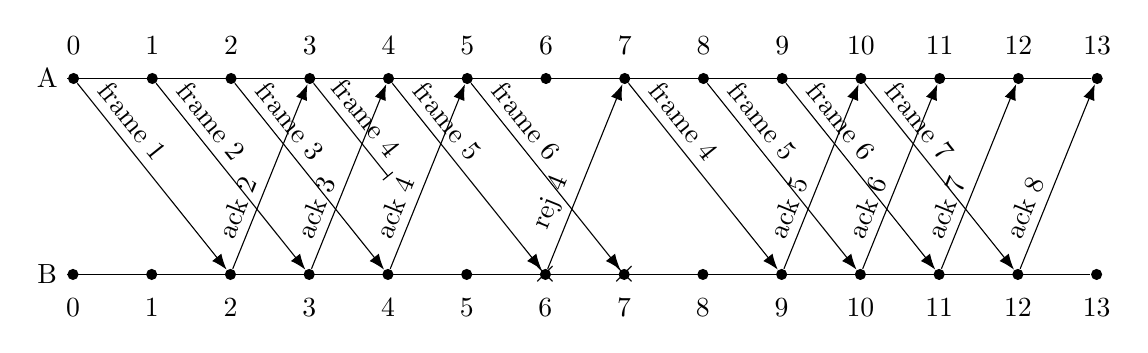
\begin{tikzpicture}
				\node at (0,0) (A) {A};
				\node (B) [below=2cm of A] {B};
				\node (A_end) [right=13cm of A] {};
				\node (B_end) [right=13cm of B] {};
				\draw (A) -- (A_end);
				\draw (B) -- (B_end);
				\foreach \x in {0,...,13} {
					\node[circle, inner sep=0.5mm, fill] (A_\x) [right=\x cm of A.east] {};
					\node[above=1mm of A_\x] {\x};
					\node[circle, inner sep=0.5mm, fill] (B_\x) [right=\x cm of B.east] {};
					\node[below=1mm of B_\x] {\x};
				}

				\draw[-{Latex[length=2mm]}] (A_0) -- (B_2)
				node[midway, sloped, above left] {frame 1};
				\draw[-{Latex[length=2mm]}] (B_2) -- (A_3)
				node[midway, sloped, above left] {ack 2};

				\draw[-{Latex[length=2mm]}] (A_1) -- (B_3)
				node[midway, sloped, above left] {frame 2};
				\draw[-{Latex[length=2mm]}] (B_3) -- (A_4)
				node[midway, sloped, above left] {ack 3};

				\draw[-{Latex[length=2mm]}] (A_2) -- (B_4)
				node[midway, sloped, above left] {frame 3};
				\draw[-{Latex[length=2mm]}] (B_4) -- (A_5)
				node[midway, sloped, above left] {ack 4};

				\draw[-|] (A_3) -- ($(A_3)!0.5!(B_5)$)
				node[midway, sloped, above] {frame 4};

				\draw[-{Latex[length=2mm]}] (A_4) -- (B_6)
				node[midway, sloped, above left] {frame 5};
				\draw[-{Latex[length=2mm]}] (B_6) -- (A_7)
				node[midway, sloped, above left] {rej 4};
				\node[below=-0.342cm of B_6] {\large\(\times\)};

				\draw[-{Latex[length=2mm]}] (A_5) -- (B_7)
				node[midway, sloped, above left] {frame 6};
				\node[below=-0.342cm of B_7] {\large\(\times\)};

				\draw[-{Latex[length=2mm]}] (A_7) -- (B_9)
				node[midway, sloped, above left] {frame 4};
				\draw[-{Latex[length=2mm]}] (B_9) -- (A_10)
				node[midway, sloped, above left] {ack 5};

				\draw[-{Latex[length=2mm]}] (A_8) -- (B_10)
				node[midway, sloped, above left] {frame 5};
				\draw[-{Latex[length=2mm]}] (B_10) -- (A_11)
				node[midway, sloped, above left] {ack 6};

				\draw[-{Latex[length=2mm]}] (A_9) -- (B_11)
				node[midway, sloped, above left] {frame 6};
				\draw[-{Latex[length=2mm]}] (B_11) -- (A_12)
				node[midway, sloped, above left] {ack 7};

				\draw[-{Latex[length=2mm]}] (A_10) -- (B_12)
				node[midway, sloped, above left] {frame 7};
				\draw[-{Latex[length=2mm]}] (B_12) -- (A_13)
				node[midway, sloped, above left] {ack 8};

			\end{tikzpicture}
		\end{figure}

		\item % 2.2
		The sequence number values that switch A will get from the first acknowledgement until the final acknowledgement is 2, 3, 4, 4, 5, 6, 7, 8.
	\end{enumerate}
\end{enumerate}

\end{document}
